\documentclass[a4paper,11pt]{article}
\usepackage[a4paper, margin=8em]{geometry}

% usa i pacchetti per la scrittura in italiano
\usepackage[french,italian]{babel}
\usepackage[T1]{fontenc}
\usepackage[utf8]{inputenc}
\frenchspacing 

% usa i pacchetti per la formattazione matematica
\usepackage{amsmath, amssymb, amsthm, amsfonts}

% usa altri pacchetti
\usepackage{gensymb}
\usepackage{hyperref}
\usepackage{standalone}

\usepackage{colortbl}

\usepackage{xstring}
\usepackage{karnaugh-map}

% imposta il titolo
\title{Appunti Programmazione Avanzata}
\author{Luca Seggiani}
\date{2025}

% imposta lo stile
% usa helvetica
\usepackage[scaled]{helvet}
% usa palatino
\usepackage{palatino}
% usa un font monospazio guardabile
\usepackage{lmodern}

\renewcommand{\rmdefault}{ppl}
\renewcommand{\sfdefault}{phv}
\renewcommand{\ttdefault}{lmtt}

% circuiti
\usepackage{circuitikz}
\usetikzlibrary{babel}

% testo cerchiato
\newcommand*\circled[1]{\tikz[baseline=(char.base)]{
            \node[shape=circle,draw,inner sep=2pt] (char) {#1};}}

% disponi il titolo
\makeatletter
\renewcommand{\maketitle} {
	\begin{center} 
		\begin{minipage}[t]{.8\textwidth}
			\textsf{\huge\bfseries \@title} 
		\end{minipage}%
		\begin{minipage}[t]{.2\textwidth}
			\raggedleft \vspace{-1.65em}
			\textsf{\small \@author} \vfill
			\textsf{\small \@date}
		\end{minipage}
		\par
	\end{center}

	\thispagestyle{empty}
	\pagestyle{fancy}
}
\makeatother

% disponi teoremi
\usepackage{tcolorbox}
\newtcolorbox[auto counter, number within=section]{theorem}[2][]{%
	colback=blue!10, 
	colframe=blue!40!black, 
	sharp corners=northwest,
	fonttitle=\sffamily\bfseries, 
	title=Teorema~\thetcbcounter: #2, 
	#1
}

% disponi definizioni
\newtcolorbox[auto counter, number within=section]{definition}[2][]{%
	colback=red!10,
	colframe=red!40!black,
	sharp corners=northwest,
	fonttitle=\sffamily\bfseries,
	title=Definizione~\thetcbcounter: #2,
	#1
}

% disponi codice
\usepackage{listings}
\usepackage[table]{xcolor}

\definecolor{codegreen}{rgb}{0,0.6,0}
\definecolor{codegray}{rgb}{0.5,0.5,0.5}
\definecolor{codepurple}{rgb}{0.58,0,0.82}
\definecolor{backcolour}{rgb}{0.95,0.95,0.92}

\lstdefinestyle{codestyle}{
		backgroundcolor=\color{black!5}, 
		commentstyle=\color{codegreen},
		keywordstyle=\bfseries\color{magenta},
		numberstyle=\sffamily\tiny\color{black!60},
		stringstyle=\color{green!50!black},
		basicstyle=\ttfamily\footnotesize,
		breakatwhitespace=false,         
		breaklines=true,                 
		captionpos=b,                    
		keepspaces=true,                 
		numbers=left,                    
		numbersep=5pt,                  
		showspaces=false,                
		showstringspaces=false,
		showtabs=false,                  
		tabsize=2
}

\lstdefinestyle{shellstyle}{
		backgroundcolor=\color{black!5}, 
		basicstyle=\ttfamily\footnotesize\color{black}, 
		commentstyle=\color{black}, 
		keywordstyle=\color{black},
		numberstyle=\color{black!5},
		stringstyle=\color{black}, 
		showspaces=false,
		showstringspaces=false, 
		showtabs=false, 
		tabsize=2, 
		numbers=none, 
		breaklines=true
}


\lstdefinelanguage{assembler}{ 
  keywords={AAA, AAD, AAM, AAS, ADC, ADCB, ADCW, ADCL, ADD, ADDB, ADDW, ADDL, AND, ANDB, ANDW, ANDL,
        ARPL, BOUND, BSF, BSFL, BSFW, BSR, BSRL, BSRW, BSWAP, BT, BTC, BTCB, BTCW, BTCL, BTR, 
        BTRB, BTRW, BTRL, BTS, BTSB, BTSW, BTSL, CALL, CBW, CDQ, CLC, CLD, CLI, CLTS, CMC, CMP,
        CMPB, CMPW, CMPL, CMPS, CMPSB, CMPSD, CMPSW, CMPXCHG, CMPXCHGB, CMPXCHGW, CMPXCHGL,
        CMPXCHG8B, CPUID, CWDE, DAA, DAS, DEC, DECB, DECW, DECL, DIV, DIVB, DIVW, DIVL, ENTER,
        HLT, IDIV, IDIVB, IDIVW, IDIVL, IMUL, IMULB, IMULW, IMULL, IN, INB, INW, INL, INC, INCB,
        INCW, INCL, INS, INSB, INSD, INSW, INT, INT3, INTO, INVD, INVLPG, IRET, IRETD, JA, JAE,
        JB, JBE, JC, JCXZ, JE, JECXZ, JG, JGE, JL, JLE, JMP, JNA, JNAE, JNB, JNBE, JNC, JNE, JNG,
        JNGE, JNL, JNLE, JNO, JNP, JNS, JNZ, JO, JP, JPE, JPO, JS, JZ, LAHF, LAR, LCALL, LDS,
        LEA, LEAVE, LES, LFS, LGDT, LGS, LIDT, LMSW, LOCK, LODSB, LODSD, LODSW, LOOP, LOOPE,
        LOOPNE, LSL, LSS, LTR, MOV, MOVB, MOVW, MOVL, MOVSB, MOVSD, MOVSW, MOVSX, MOVSXB,
        MOVSXW, MOVSXL, MOVZX, MOVZXB, MOVZXW, MOVZXL, MUL, MULB, MULW, MULL, NEG, NEGB, NEGW,
        NEGL, NOP, NOT, NOTB, NOTW, NOTL, OR, ORB, ORW, ORL, OUT, OUTB, OUTW, OUTL, OUTSB, OUTSD,
        OUTSW, POP, POPL, POPW, POPB, POPA, POPAD, POPF, POPFD, PUSH, PUSHL, PUSHW, PUSHB, PUSHA, 
				PUSHAD, PUSHF, PUSHFD, RCL, RCLB, RCLW, MOVSL, MOVSB, MOVSW, STOSL, STOSB, STOSW, LODSB, LODSW,
				LODSL, INSB, INSW, INSL, OUTSB, OUTSL, OUTSW
        RCLL, RCR, RCRB, RCRW, RCRL, RDMSR, RDPMC, RDTSC, REP, REPE, REPNE, RET, ROL, ROLB, ROLW,
        ROLL, ROR, RORB, RORW, RORL, SAHF, SAL, SALB, SALW, SALL, SAR, SARB, SARW, SARL, SBB,
        SBBB, SBBW, SBBL, SCASB, SCASD, SCASW, SETA, SETAE, SETB, SETBE, SETC, SETE, SETG, SETGE,
        SETL, SETLE, SETNA, SETNAE, SETNB, SETNBE, SETNC, SETNE, SETNG, SETNGE, SETNL, SETNLE,
        SETNO, SETNP, SETNS, SETNZ, SETO, SETP, SETPE, SETPO, SETS, SETZ, SGDT, SHL, SHLB, SHLW,
        SHLL, SHLD, SHR, SHRB, SHRW, SHRL, SHRD, SIDT, SLDT, SMSW, STC, STD, STI, STOSB, STOSD,
        STOSW, STR, SUB, SUBB, SUBW, SUBL, TEST, TESTB, TESTW, TESTL, VERR, VERW, WAIT, WBINVD,
        XADD, XADDB, XADDW, XADDL, XCHG, XCHGB, XCHGW, XCHGL, XLAT, XLATB, XOR, XORB, XORW, XORL},
  keywordstyle=\color{blue}\bfseries,
  ndkeywordstyle=\color{darkgray}\bfseries,
  identifierstyle=\color{black},
  sensitive=false,
  comment=[l]{\#},
  morecomment=[s]{/*}{*/},
  commentstyle=\color{purple}\ttfamily,
  stringstyle=\color{red}\ttfamily,
  morestring=[b]',
  morestring=[b]"
}

\lstset{language=java, style=codestyle}

% disponi sezioni
\usepackage{titlesec}

\titleformat{\section}
	{\sffamily\Large\bfseries} 
	{\thesection}{1em}{} 
\titleformat{\subsection}
	{\sffamily\large\bfseries}   
	{\thesubsection}{1em}{} 
\titleformat{\subsubsection}
	{\sffamily\normalsize\bfseries} 
	{\thesubsubsection}{1em}{}

% tikz
\usepackage{tikz}

% float
\usepackage{float}

% grafici
\usepackage{pgfplots}
\pgfplotsset{width=10cm,compat=1.9}

% disponi alberi
\usepackage{forest}

\forestset{
	rectstyle/.style={
		for tree={rectangle,draw,font=\large\sffamily}
	},
	roundstyle/.style={
		for tree={circle,draw,font=\large}
	}
}

% disponi algoritmi
\usepackage{algorithm}
\usepackage{algorithmic}
\makeatletter
\renewcommand{\ALG@name}{Algoritmo}
\makeatother

% disponi numeri di pagina
\usepackage{fancyhdr}
\fancyhf{} 
\fancyfoot[L]{\sffamily{\thepage}}

\makeatletter
\fancyhead[L]{\raisebox{1ex}[0pt][0pt]{\sffamily{\@title \ \@date}}} 
\fancyhead[R]{\raisebox{1ex}[0pt][0pt]{\sffamily{\@author}}}
\makeatother

\begin{document}

\pagestyle{fancy}
\thispagestyle{empty}
\renewcommand{\thispagestyle}[1]{}

\maketitle
\documentclass[a4paper,11pt]{article}
\usepackage[a4paper, margin=8em]{geometry}

% usa i pacchetti per la scrittura in italiano
\usepackage[french,italian]{babel}
\usepackage[T1]{fontenc}
\usepackage[utf8]{inputenc}
\frenchspacing 

% usa i pacchetti per la formattazione matematica
\usepackage{amsmath, amssymb, amsthm, amsfonts}

% usa altri pacchetti
\usepackage{gensymb}
\usepackage{hyperref}
\usepackage{standalone}

\usepackage{colortbl}

\usepackage{xstring}
\usepackage{karnaugh-map}

% imposta il titolo
\title{Appunti Programmazione Avanzata}
\author{Luca Seggiani}
\date{2025}

% imposta lo stile
% usa helvetica
\usepackage[scaled]{helvet}
% usa palatino
\usepackage{palatino}
% usa un font monospazio guardabile
\usepackage{lmodern}

\renewcommand{\rmdefault}{ppl}
\renewcommand{\sfdefault}{phv}
\renewcommand{\ttdefault}{lmtt}

% circuiti
\usepackage{circuitikz}
\usetikzlibrary{babel}

% testo cerchiato
\newcommand*\circled[1]{\tikz[baseline=(char.base)]{
            \node[shape=circle,draw,inner sep=2pt] (char) {#1};}}

% disponi il titolo
\makeatletter
\renewcommand{\maketitle} {
	\begin{center} 
		\begin{minipage}[t]{.8\textwidth}
			\textsf{\huge\bfseries \@title} 
		\end{minipage}%
		\begin{minipage}[t]{.2\textwidth}
			\raggedleft \vspace{-1.65em}
			\textsf{\small \@author} \vfill
			\textsf{\small \@date}
		\end{minipage}
		\par
	\end{center}

	\thispagestyle{empty}
	\pagestyle{fancy}
}
\makeatother

% disponi teoremi
\usepackage{tcolorbox}
\newtcolorbox[auto counter, number within=section]{theorem}[2][]{%
	colback=blue!10, 
	colframe=blue!40!black, 
	sharp corners=northwest,
	fonttitle=\sffamily\bfseries, 
	title=Teorema~\thetcbcounter: #2, 
	#1
}

% disponi definizioni
\newtcolorbox[auto counter, number within=section]{definition}[2][]{%
	colback=red!10,
	colframe=red!40!black,
	sharp corners=northwest,
	fonttitle=\sffamily\bfseries,
	title=Definizione~\thetcbcounter: #2,
	#1
}

% disponi codice
\usepackage{listings}
\usepackage[table]{xcolor}

\definecolor{codegreen}{rgb}{0,0.6,0}
\definecolor{codegray}{rgb}{0.5,0.5,0.5}
\definecolor{codepurple}{rgb}{0.58,0,0.82}
\definecolor{backcolour}{rgb}{0.95,0.95,0.92}

\lstdefinestyle{codestyle}{
		backgroundcolor=\color{black!5}, 
		commentstyle=\color{codegreen},
		keywordstyle=\bfseries\color{magenta},
		numberstyle=\sffamily\tiny\color{black!60},
		stringstyle=\color{green!50!black},
		basicstyle=\ttfamily\footnotesize,
		breakatwhitespace=false,         
		breaklines=true,                 
		captionpos=b,                    
		keepspaces=true,                 
		numbers=left,                    
		numbersep=5pt,                  
		showspaces=false,                
		showstringspaces=false,
		showtabs=false,                  
		tabsize=2
}

\lstdefinestyle{shellstyle}{
		backgroundcolor=\color{black!5}, 
		basicstyle=\ttfamily\footnotesize\color{black}, 
		commentstyle=\color{black}, 
		keywordstyle=\color{black},
		numberstyle=\color{black!5},
		stringstyle=\color{black}, 
		showspaces=false,
		showstringspaces=false, 
		showtabs=false, 
		tabsize=2, 
		numbers=none, 
		breaklines=true
}


\lstdefinelanguage{assembler}{ 
  keywords={AAA, AAD, AAM, AAS, ADC, ADCB, ADCW, ADCL, ADD, ADDB, ADDW, ADDL, AND, ANDB, ANDW, ANDL,
        ARPL, BOUND, BSF, BSFL, BSFW, BSR, BSRL, BSRW, BSWAP, BT, BTC, BTCB, BTCW, BTCL, BTR, 
        BTRB, BTRW, BTRL, BTS, BTSB, BTSW, BTSL, CALL, CBW, CDQ, CLC, CLD, CLI, CLTS, CMC, CMP,
        CMPB, CMPW, CMPL, CMPS, CMPSB, CMPSD, CMPSW, CMPXCHG, CMPXCHGB, CMPXCHGW, CMPXCHGL,
        CMPXCHG8B, CPUID, CWDE, DAA, DAS, DEC, DECB, DECW, DECL, DIV, DIVB, DIVW, DIVL, ENTER,
        HLT, IDIV, IDIVB, IDIVW, IDIVL, IMUL, IMULB, IMULW, IMULL, IN, INB, INW, INL, INC, INCB,
        INCW, INCL, INS, INSB, INSD, INSW, INT, INT3, INTO, INVD, INVLPG, IRET, IRETD, JA, JAE,
        JB, JBE, JC, JCXZ, JE, JECXZ, JG, JGE, JL, JLE, JMP, JNA, JNAE, JNB, JNBE, JNC, JNE, JNG,
        JNGE, JNL, JNLE, JNO, JNP, JNS, JNZ, JO, JP, JPE, JPO, JS, JZ, LAHF, LAR, LCALL, LDS,
        LEA, LEAVE, LES, LFS, LGDT, LGS, LIDT, LMSW, LOCK, LODSB, LODSD, LODSW, LOOP, LOOPE,
        LOOPNE, LSL, LSS, LTR, MOV, MOVB, MOVW, MOVL, MOVSB, MOVSD, MOVSW, MOVSX, MOVSXB,
        MOVSXW, MOVSXL, MOVZX, MOVZXB, MOVZXW, MOVZXL, MUL, MULB, MULW, MULL, NEG, NEGB, NEGW,
        NEGL, NOP, NOT, NOTB, NOTW, NOTL, OR, ORB, ORW, ORL, OUT, OUTB, OUTW, OUTL, OUTSB, OUTSD,
        OUTSW, POP, POPL, POPW, POPB, POPA, POPAD, POPF, POPFD, PUSH, PUSHL, PUSHW, PUSHB, PUSHA, 
				PUSHAD, PUSHF, PUSHFD, RCL, RCLB, RCLW, MOVSL, MOVSB, MOVSW, STOSL, STOSB, STOSW, LODSB, LODSW,
				LODSL, INSB, INSW, INSL, OUTSB, OUTSL, OUTSW
        RCLL, RCR, RCRB, RCRW, RCRL, RDMSR, RDPMC, RDTSC, REP, REPE, REPNE, RET, ROL, ROLB, ROLW,
        ROLL, ROR, RORB, RORW, RORL, SAHF, SAL, SALB, SALW, SALL, SAR, SARB, SARW, SARL, SBB,
        SBBB, SBBW, SBBL, SCASB, SCASD, SCASW, SETA, SETAE, SETB, SETBE, SETC, SETE, SETG, SETGE,
        SETL, SETLE, SETNA, SETNAE, SETNB, SETNBE, SETNC, SETNE, SETNG, SETNGE, SETNL, SETNLE,
        SETNO, SETNP, SETNS, SETNZ, SETO, SETP, SETPE, SETPO, SETS, SETZ, SGDT, SHL, SHLB, SHLW,
        SHLL, SHLD, SHR, SHRB, SHRW, SHRL, SHRD, SIDT, SLDT, SMSW, STC, STD, STI, STOSB, STOSD,
        STOSW, STR, SUB, SUBB, SUBW, SUBL, TEST, TESTB, TESTW, TESTL, VERR, VERW, WAIT, WBINVD,
        XADD, XADDB, XADDW, XADDL, XCHG, XCHGB, XCHGW, XCHGL, XLAT, XLATB, XOR, XORB, XORW, XORL},
  keywordstyle=\color{blue}\bfseries,
  ndkeywordstyle=\color{darkgray}\bfseries,
  identifierstyle=\color{black},
  sensitive=false,
  comment=[l]{\#},
  morecomment=[s]{/*}{*/},
  commentstyle=\color{purple}\ttfamily,
  stringstyle=\color{red}\ttfamily,
  morestring=[b]',
  morestring=[b]"
}

\lstset{language=assembler, style=codestyle}

% disponi sezioni
\usepackage{titlesec}

\titleformat{\section}
	{\sffamily\Large\bfseries} 
	{\thesection}{1em}{} 
\titleformat{\subsection}
	{\sffamily\large\bfseries}   
	{\thesubsection}{1em}{} 
\titleformat{\subsubsection}
	{\sffamily\normalsize\bfseries} 
	{\thesubsubsection}{1em}{}

% tikz
\usepackage{tikz}

% float
\usepackage{float}

% grafici
\usepackage{pgfplots}
\pgfplotsset{width=10cm,compat=1.9}

% disponi alberi
\usepackage{forest}

\forestset{
	rectstyle/.style={
		for tree={rectangle,draw,font=\large\sffamily}
	},
	roundstyle/.style={
		for tree={circle,draw,font=\large}
	}
}

% disponi algoritmi
\usepackage{algorithm}
\usepackage{algorithmic}
\makeatletter
\renewcommand{\ALG@name}{Algoritmo}
\makeatother

% disponi numeri di pagina
\usepackage{fancyhdr}
\fancyhf{} 
\fancyfoot[L]{\sffamily{\thepage}}

\makeatletter
\fancyhead[L]{\raisebox{1ex}[0pt][0pt]{\sffamily{\@title \ \@date}}} 
\fancyhead[R]{\raisebox{1ex}[0pt][0pt]{\sffamily{\@author}}}
\makeatother

\begin{document}
% sezione (data)
\section{Lezione del 23-09-25}

% stili pagina
\thispagestyle{empty}
\pagestyle{fancy}

% testo
\subsection{Introduzione}
Il corso di programmazione avanzata si pone di approfondire gli aspetti di programmazione \textit{orientata agli oggetti} (\textbf{OOP}) e \textit{concorrente}, sfruttando sia come strumento che come fine il linguaggio di programmazione \textbf{Java}.
Parleremo sia di programmazione desktop che applicazioni in rete (cioè servizi per pagine Web).

\subsubsection{Cenni storici}
Java nasce nei primi anni '90 come \textit{Oak} all'interno della \textit{Sun Microsystems} (poi acquisita da Oracle).

L'idea originale del progetto era quella di realizzare un linguaggio per la programmazione di dispositivi di elettronica di consumo.
Per questo motivo una delle prime prerogative del progetto era che il linguaggio potesse creare programmi che giravano su una variegata gamma di piattaforme hardware (il cosiddetto paradigma \textbf{WORA}, \textit{Write Once, Run Anywhere}).

Con l'avvento del Web e delle applicazioni distribuite in modello client-server, l'obiettivo del progetto virò verso la creazione di un linguaggio che potesse essere eseguito sui client, all'interno dei browser (nei cosiddetti \textit{applet}), a scapito dell'architettura o il S/O locale (browser Netscape su architetture non-Intel e S/O Unix come browser Explorer su architetture Intel e S/O Microsoft).

Oggi questo tipo di uso è in declino, ma il linguaggio Java rimane estremamente popolare per lo sviluppo di applicazioni desktop/mobile, e in contesto sopratutto aziendale per lo sviluppo di applicazioni lato server.

\subsubsection{Versioni}
Possiamo individuare alcune versioni di rilevo dello standard Java.
\begin{itemize}
	\item Nel 1996 viene lanciata la JDK 1.0 (\textit{Java Development Kit}), prima versione del linguaggio;
	\item Nel 1998 viene lanciata la J2SE 1.2, da cui la denominazione \textit{Java 2}, rimasta fino alla 5.0 del 2004 (fra l'altro slegata in nome dalla versione precedente, la 1.4);
	\item Dal 2006 vengono usate le denominazioni Java SE 6 e successive, ed è stato adottato un modello di rilascio periodico (da Java SE 9 annuale).
		Questo è più o meno in corrispondenza dell'acquisto da parte di Oracle di Sun Microsystems, avvenuto nel 2010 (la prima versione lanciata sotto la Oracle fu Java SE 7).
\end{itemize}

Nel progetto originale della Sun Microsystems erano previste più \textit{edizioni} di Java, fra cui:
\begin{itemize}
	\item Java \textbf{ME}, cioè \textit{Micro Edition}, che mirava a piattaforme con risorse limitate;
	\item Java \textbf{SE}, cioè \textit{Standard Edition}, che mirava a piattaforme desktop;
	\item Java \textbf{EE}, cioè \textit{Enterprise Edition}, che mirava a piattaforme distribuite e in rete.
\end{itemize}

Java è fornito sia come \textbf{JDK} (come già detto \textit{Java Development Kit}), comprensivo di compilatore e strumenti di sviluppo, che come \textbf{JRE} (\textit{Java Runtime Environment}), pensato solo per l'esecuzione di applicazioni già sviluppate.

Notiamo poi che noi useremo la piattaforma \textbf{OpenJDK}, implementazione open source del JDK lanciata da Sun Microsystems nel 2006, prima dell'acquisizione da parte di Oracle, e ancora oggi mantenuta da Oracle ma comunque mantenuta open source. 

\subsubsection{Natura del Java}
I design goal di Java sono i seguenti: 
\begin{itemize}
	\item Semplice, paradigma orientato agli oggetti e familiare per gli sviluppatori di linguaggi precedenti (si pensi alla famiglia C/C++, con cui condivide sintassi e diversi costrutti);
	\item Robusto e sicuro, in particolare riguardo alla memoria (non sono presenti meccanismi come i puntatori, e la gestione della memoria è quindi \textit{sicura} e largamente fuori dalle mani del programmatore);
	\item \textit{Architecture-neutral}, cioè neutrale all'architettura e portatile su una vasta gamma di piattaforme (come già detto, paradigma \textit{WORA}). In questo, la specifica non contiene ambiguità (i tipi, ad esempio, sono standardizzati in dimensioni, a differenza del C++ che è \textit{platform-dependent}).

		Il codice sorgente Java viene compilato nel cosiddetto \textbf{bytecode}, una sorta di codice macchina che viene eseguito sulla \textbf{JVM}, una macchina virtuale basata sullo \textit{stack} piuttosto che su \textit{registri}, e agnostica al livello fisico sottostante;
	\item Alte prestazioni, difficili da ottenere a causa della sua natura sostanzialmente interpretata, ma comunque quasi paragonabili nelle ultime versioni a codice scritto con linguaggi come C/C++, sopratutto nel caso di codice che viene ripetuto molte volte.
		Questo è reso possibile anche dall'uso di tecnologie di compilazione \textbf{JIT} (compilazione \textit{Just In Time}).

		Come nota storica, vediamo che sono state sviluppate implementazioni hardware della JVM, oggi non più particolarmente in voga;
	\item Interpretato, \textit{threaded}, cioè ottimizzato per l'esecuzione su sistemi \textit{multithreaded}, e dinamico per quanto riguarda il collegamento delle librerie, che viene effettuato a tempo di esecuzione.
\end{itemize}

Abbiamo quindi che le differenza principali fra i linguaggi C/C++ a cui siamo abituati e il Java sono:
\begin{itemize}
	\item La natura dinamica del Java (anche le classi possono essere caricate a tempo di esecuzione);
	\item Il supporto nativo per il multithreading, che in Java è praticamente immediato, mentre in C++ richiede API e tecniche di programmazione considerevolmente più complesse.
\end{itemize}

\subsubsection{Java e Android}
Un caso di applicazione di Java degno di nota è quello dello sviluppo di applicazioni per il sistema operativo Android.

Android era infatti fornito nelle prime versioni della macchina virtuale \textbf{Dalvik}, basata sui registri, che esegue codice Java compilato in un bytecode apposito, appunto il codice \textit{Dalvik} (da cui \lstinline|.dex|, \textit{Dalvin EXecutable}).

Il supporto per la macchina Dalvik è rimasto in Android fino alla versione 4.4 \textit{KitKat}, ed è stato seguito nella 5.0 \textit{Lollipop} da \textbf{ART} (\textit{Android RunTime}), che usa lo stesso bytecode e gli stessi eseguibili, ma con diverse ottimizzazioni.

Notiamo poi che oggi (dal 2019) Android è una piattaforma \textit{Kotlin-first}, cioè orientata al linguaggio "successore" del Java, il \textbf{Kotlin}.

\subsection{Ciao mondo in Java}
Possiamo quindi vedere il nostro primo programma di esempio in Java.
\begin{lstlisting}[language=java, style=codestyle]	
class Main {
	public static void main(String[] args) {
		System.out.println("C# is better");
	}
}
\end{lstlisting}

Vediamo come tutto sta necessariamente dentro una classe, qui la classe \lstinline|Main|, che definisce un metodo, qui il metodo \lstinline|main()|.

Questo metodo è specifico (come il \lstinline|main()| del C/C++), viene eseguito quando la classe che lo possiede è invocata come programma, e ha come argomento la lista degli argomenti programma \lstinline|String[] args|, dove le quadre definiscono un'array come per la normale sintassi c-like.
Inoltre, il metodo \lstinline|main()| è dichiarato come:
\begin{itemize}
	\item \lstinline|public|, cioè chiunque può invocarlo;
	\item \lstinline|static|, cioè appartiene alla definizione di classe stessa, e non ad una particolare istanza di classe.
\end{itemize}

Da qui usiamo la funzione di libreria \lstinline|println| per stampare un messaggio a video.

Possiamo compilare questo codice inserendolo in un file col nome della classe definita, \lstinline|Main.java|, e compilare come:
\begin{lstlisting}[style=shellstyle]
javac Main.json
\end{lstlisting}
Questo creerà un nuovo file, \lstinline|Main.class|, contenente appunto la classe \lstinline|Main|.
A questo punto si esegue come:
\begin{lstlisting}[style=shellstyle]
java Main
\end{lstlisting}
notando che si riporta solo il nome della classe, senza l'estensione \lstinline|.java|.

\subsection{Tipi del Java}
Il Java è un linguaggio fortemente tipizzato dove ogni oggetto ha un tipo.
In particolare notiamo fra tipi \textbf{primitivi} e di \textbf{riferimento}.

\newpage

\begin{itemize}
	\item I tipi \textbf{primitivi} sono i classici tipi di dato disponibili negli altri linguaggi:
\begin{lstlisting}[language=java, style=codestyle]	
int x;
float y = 5.6;
double pippo = 3.2 + Math.sqrt(7.4);
int i1, i2, i3;
char a = 'a';
// String s = "Also try Kotlin";
/* const int VAL; no ! */ 
static final int VAL; // e' effettivamente costante
\end{lstlisting}
La lista completa dei tipi è la seguente:
	\begin{table}[H]
		\center \rowcolors{2}{white}{black!10}
		\begin{tabular} { c | c }
			\bfseries Tipo & \bfseries Descrizione \\
			\hline
			\lstinline|boolean| & Un booleano \lstinline|true| o \lstinline|false| \\ 
			\lstinline|char| & Un carattere, cioè un \textit{codepoint} UTF-16 su 16 bit \\ 
			\lstinline|byte| & Un intero su 8 bit \\ 
			\lstinline|short| & Un intero su 16 bit \\ 
			\lstinline|int| & Un intero su 32 bit \\ 
			\lstinline|long| & Un intero su 64 bit \\ 
			\lstinline|float| & Un numero in virgola mobile su 32 bit come definito da IEEE 754 \\ 
			\lstinline|double| & Un numero in virgola mobile su 64 bit come definito da IEEE 754 \\ 
		\end{tabular}
	\end{table}
		Notiamo innanzitutto che il Java adotta la codifica UTF-8 per le stringhe e UTF-16 per i caratteri. Ricordiamo poi che, come già detto, i tipi del Java (ad esempio i tipi numerici) hanno dimensione fissata dalla specifica e non \textit{platform-specific}.

	Vediamo poi che la parola chiave \lstinline|const| non è implementata in Java (anche se è comunque riservata), mentre sono disponibili le parole chiave \lstinline|static| e \lstinline|final|. In particolare questa assegna a variabili valori finali, cioè che non possono più essere alterati.

	I valori non inizializzati in Java vengono lasciati in uno stato \lstinline|undefined|, possono restare tali fino alla definizione, ma se si prova ad usarli prima il compilatore lancia un errore.

	Per ogni tipo primitivo esiste poi un corrispondente \textit{tipo oggetto}, cioè sostanzialmente una classe \textit{wrapper} per quel tipo di primitivo. 

	\par\medskip
	\textbf{\textsf{Conversioni fra tipi}} \\
	\noindent
	La conversione fra tipi primitivi e oggetto corrispondenti è automatica.
	Sono poi previste le conversioni implicite fra tipi primitivi secondo i meccanismi che ci aspettiamo:

	\begin{center}	
		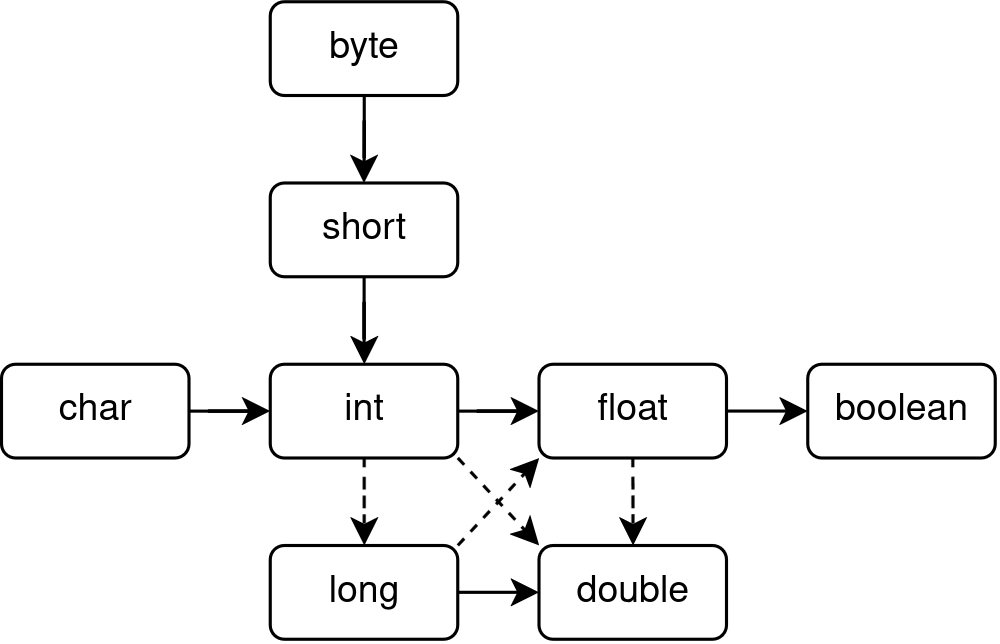
\includegraphics[scale=0.3]{../figures/conversioni_implicite.png}
	\end{center}

	Per effettuare cast nelle direzioni opposte a quelle previste dalle conversioni implicite si usano le conversioni esplicite secondo la solita sintassi:
\begin{lstlisting}[language=java, style=codestyle]	
float pi = 3.14;
int engineer_pi = (int) pi; // engineer_pi = 3
\end{lstlisting}

	\item I tipi di \textbf{riferimento} comprendono:
		\begin{itemize}
			\item Array;
			\item Classi;
			\item Interfacce.
		\end{itemize}
\end{itemize}

\subsubsection{Costrutti del Java}
Il Java comprende tutti i costrutti condizionali e di ripetizione a cui siamo abituati.
Notiamo in particolare la presenza del costrutto \textit{for-each} disponibile come:
\begin{lstlisting}[language=java, style=codestyle]	
for(tipo variabile : espressione_insieme) {
	// corpo
}
\end{lstlisting}
che itera sugli elementi dell'oggetto \lstinline|set_expression| instanziandoli ogni volta nell'oggetto \lstinline|variabile|.

Vediamo quindi tutti i costrutti disponibili:

\noindent
\begin{minipage}[t]{0.45\textwidth}
\begin{table}[H]
	\center 
	\begin{tabular} { c | p{.1cm} p{5cm} }
		\bfseries Costrutto & \bfseries Sintassi \\ 
		\hline 
\lstinline|if-else| & & \begin{lstlisting}[language=java, style=codestyle]	
if(espressione) {
	// vera
} else {
	// falsa
}
\end{lstlisting} \\
\lstinline|switch| & & \begin{lstlisting}[language=java, style=codestyle]	
switch(espressione) {
	case a: // caso a
	case b: // caso b
	// ...
	default: // caso default
}
\end{lstlisting} \\
\lstinline|while| & & \begin{lstlisting}[language=java, style=codestyle]	
while(espressione) {
	// corpo
}
\end{lstlisting} \\
\lstinline|do-while| & & \begin{lstlisting}[language=java, style=codestyle]	
do {
	// corpo
} while(espressione);
\end{lstlisting} \\
	\end{tabular}
\end{table}
\end{minipage}%
\hfill
\begin{minipage}[t]{0.45\textwidth}
\begin{table}[H]
	\center 
	\begin{tabular} { c | p{.1cm} p{5cm} }
		\bfseries Costrutto & \bfseries Sintassi \\ 
		\hline 
\lstinline|for| & & \begin{lstlisting}[language=java, style=codestyle]	
for(espressione; espressione; espressione) {
	// corpo
}
\end{lstlisting} \\
\lstinline|for-each| & & \begin{lstlisting}[language=java, style=codestyle]	
for(tipo variabile : espressione_insieme) {
	// corpo
}
\end{lstlisting} \\
\lstinline|break| & & \begin{lstlisting}[language=java, style=codestyle]	
break;
\end{lstlisting} \\
\lstinline|continue| & & \begin{lstlisting}[language=java, style=codestyle]	
continue;
\end{lstlisting} \\
	\end{tabular}
\end{table}
\end{minipage}

\subsubsection{Classe \lstinline|System|}
\lstinline|System| è una classe delle librerie Java dotata di 3 campi per la gestione degli stream di I/O:
\begin{itemize}
	\item \lstinline|System.in|, che gestisce il flusso di ingresso (tastiera).
		Per l'ingresso inglobiamo lo stream \lstinline|System.in| all'interno della classe \lstinline|Scanner| come segue:
\begin{lstlisting}[language=java, style=codestyle]	
Scanner s = new Scanner(System.in);
\end{lstlisting}
A questo punto possiamo usare i metodi della classe scanner come \lstinline|next()| (che si ferma alla parola) e \lstinline|nextLine()| (che si ferma alla riga) per leggere dallo stream.
Vediamo che la classe \lstinline|Scanner| è la prima che incontriamo a non essere inclusa di default nel sorgente, ma che va inclusa con la direttiva \lstinline|import|:
\begin{lstlisting}[language=java, style=codestyle]	
import java.util.Scanner;

// classe main, ecc... 
\end{lstlisting}
	\item \lstinline|System.out|, che gestisce il flusso di uscita (video). Sono disponibili i metodi \lstinline|println()|, e \lstinline|print()| (che non stampa i caratteli di ritorno carrello e nuova linea);
	\item \lstinline|System.err|, che gestisce il flusso di errore (sempre video);
\end{itemize}

\subsection{Classi del Java}
In Java \textit{tutto} il codice è dentro classi.
Una classe contiene:
\begin{itemize}
	\item La definizione della struttura degli oggetti (istanze) della classe attraverso le \textit{variabili istanza};
	\item La definizione della struttura dei dati comuni ad ogni classe attraverso le \textit{variabili classe}.
\end{itemize}
Queste strutture vengono definite con:
\begin{itemize}
	\item Variabili possedute dalla classe (\textbf{campi});
	\item Codice che manipola gli oggetti, o in particolare i membri di classe (\textbf{metodi} e non \textit{funzioni});
	\item I meccanismi per la costruzione di oggetti (\textbf{costruttori}).
\end{itemize}
Variabili e funzioni di classe (cioè campi e metodi) sono anche detti \textbf{membri}.

Una classe in Java si istanzia sempre con la parola chiave \lstinline|new|, in quanto non si possono allocare classi Java sullo stack, solo sull'heap.
Abbiamo quindi che:
\begin{lstlisting}[language=java, style=codestyle]	
Classe cl1;
\end{lstlisting}
non istanzia alcuna classe, ma esiste solo come un oggetto \textit{riferimento} a oggetti di tipo \lstinline|Classe|, che colleghiamo ad un oggetto vero e proprio sull'heap come:
\begin{lstlisting}[language=java, style=codestyle]	
Classe cl1 = new Classe(/* argomenti del costruttore */);
\end{lstlisting}

Il fatto che gli oggetti dichiarati come \lstinline|Classe| sono solo riferimenti ad oggetti sull'heap significa che facendo cose come \lstinline|cl1 = cl2| stiamo solo spostando il riferimento da un oggetto all'altro, e non copiando le variabili istanza dei singoli oggetti.

Per accedere alle variabili istanza usiamo la classica notazione a punto (\lstinline|Classe.variabile|, ecc...).
Nessuno ci nega di includere riferimenti ad altre classi come membri di classi, dobbiamo solo ricordare che stiamo parlando sempre di riferimenti e non di oggetti classe veri e propri.

\subsubsection{Costruttori}
I costruttori sono sequenze di istruzioni utilizzate per definire lo stato iniziale di un oggetto in fase di instanziazione (quando viene usata la \lstinline|new|), nel caso questo sia necessario, cioè i meccanismi standard non sono sufficienti (costruttore di default nullo) o ci sono informazioni note solo al momento della \lstinline|new|.

I costruttori del Java:
\begin{itemize}
	\item Hanno lo stesso nome della classe;
	\item Non restituiscono valore;
	\item Possono essere eseguiti solo in occasione della \lstinline|new|;
	\item Possono avere 0 o più argomenti.
\end{itemize}

\end{document}

\documentclass[a4paper,11pt]{article}
\usepackage[a4paper, margin=8em]{geometry}

% usa i pacchetti per la scrittura in italiano
\usepackage[french,italian]{babel}
\usepackage[T1]{fontenc}
\usepackage[utf8]{inputenc}
\frenchspacing 

% usa i pacchetti per la formattazione matematica
\usepackage{amsmath, amssymb, amsthm, amsfonts}

% usa altri pacchetti
\usepackage{gensymb}
\usepackage{hyperref}
\usepackage{standalone}

\usepackage{colortbl}

\usepackage{xstring}
\usepackage{karnaugh-map}

% imposta il titolo
\title{Appunti Programmazione Avanzata}
\author{Luca Seggiani}
\date{2025}

% imposta lo stile
% usa helvetica
\usepackage[scaled]{helvet}
% usa palatino
\usepackage{palatino}
% usa un font monospazio guardabile
\usepackage{lmodern}

\renewcommand{\rmdefault}{ppl}
\renewcommand{\sfdefault}{phv}
\renewcommand{\ttdefault}{lmtt}

% circuiti
\usepackage{circuitikz}
\usetikzlibrary{babel}

% testo cerchiato
\newcommand*\circled[1]{\tikz[baseline=(char.base)]{
            \node[shape=circle,draw,inner sep=2pt] (char) {#1};}}

% disponi il titolo
\makeatletter
\renewcommand{\maketitle} {
	\begin{center} 
		\begin{minipage}[t]{.8\textwidth}
			\textsf{\huge\bfseries \@title} 
		\end{minipage}%
		\begin{minipage}[t]{.2\textwidth}
			\raggedleft \vspace{-1.65em}
			\textsf{\small \@author} \vfill
			\textsf{\small \@date}
		\end{minipage}
		\par
	\end{center}

	\thispagestyle{empty}
	\pagestyle{fancy}
}
\makeatother

% disponi teoremi
\usepackage{tcolorbox}
\newtcolorbox[auto counter, number within=section]{theorem}[2][]{%
	colback=blue!10, 
	colframe=blue!40!black, 
	sharp corners=northwest,
	fonttitle=\sffamily\bfseries, 
	title=Teorema~\thetcbcounter: #2, 
	#1
}

% disponi definizioni
\newtcolorbox[auto counter, number within=section]{definition}[2][]{%
	colback=red!10,
	colframe=red!40!black,
	sharp corners=northwest,
	fonttitle=\sffamily\bfseries,
	title=Definizione~\thetcbcounter: #2,
	#1
}

% disponi codice
\usepackage{listings}
\usepackage[table]{xcolor}

\definecolor{codegreen}{rgb}{0,0.6,0}
\definecolor{codegray}{rgb}{0.5,0.5,0.5}
\definecolor{codepurple}{rgb}{0.58,0,0.82}
\definecolor{backcolour}{rgb}{0.95,0.95,0.92}

\lstdefinestyle{codestyle}{
		backgroundcolor=\color{black!5}, 
		commentstyle=\color{codegreen},
		keywordstyle=\bfseries\color{magenta},
		numberstyle=\sffamily\tiny\color{black!60},
		stringstyle=\color{green!50!black},
		basicstyle=\ttfamily\footnotesize,
		breakatwhitespace=false,         
		breaklines=true,                 
		captionpos=b,                    
		keepspaces=true,                 
		numbers=left,                    
		numbersep=5pt,                  
		showspaces=false,                
		showstringspaces=false,
		showtabs=false,                  
		tabsize=2
}

\lstdefinestyle{shellstyle}{
		backgroundcolor=\color{black!5}, 
		basicstyle=\ttfamily\footnotesize\color{black}, 
		commentstyle=\color{black}, 
		keywordstyle=\color{black},
		numberstyle=\color{black!5},
		stringstyle=\color{black}, 
		showspaces=false,
		showstringspaces=false, 
		showtabs=false, 
		tabsize=2, 
		numbers=none, 
		breaklines=true
}


\lstdefinelanguage{assembler}{ 
  keywords={AAA, AAD, AAM, AAS, ADC, ADCB, ADCW, ADCL, ADD, ADDB, ADDW, ADDL, AND, ANDB, ANDW, ANDL,
        ARPL, BOUND, BSF, BSFL, BSFW, BSR, BSRL, BSRW, BSWAP, BT, BTC, BTCB, BTCW, BTCL, BTR, 
        BTRB, BTRW, BTRL, BTS, BTSB, BTSW, BTSL, CALL, CBW, CDQ, CLC, CLD, CLI, CLTS, CMC, CMP,
        CMPB, CMPW, CMPL, CMPS, CMPSB, CMPSD, CMPSW, CMPXCHG, CMPXCHGB, CMPXCHGW, CMPXCHGL,
        CMPXCHG8B, CPUID, CWDE, DAA, DAS, DEC, DECB, DECW, DECL, DIV, DIVB, DIVW, DIVL, ENTER,
        HLT, IDIV, IDIVB, IDIVW, IDIVL, IMUL, IMULB, IMULW, IMULL, IN, INB, INW, INL, INC, INCB,
        INCW, INCL, INS, INSB, INSD, INSW, INT, INT3, INTO, INVD, INVLPG, IRET, IRETD, JA, JAE,
        JB, JBE, JC, JCXZ, JE, JECXZ, JG, JGE, JL, JLE, JMP, JNA, JNAE, JNB, JNBE, JNC, JNE, JNG,
        JNGE, JNL, JNLE, JNO, JNP, JNS, JNZ, JO, JP, JPE, JPO, JS, JZ, LAHF, LAR, LCALL, LDS,
        LEA, LEAVE, LES, LFS, LGDT, LGS, LIDT, LMSW, LOCK, LODSB, LODSD, LODSW, LOOP, LOOPE,
        LOOPNE, LSL, LSS, LTR, MOV, MOVB, MOVW, MOVL, MOVSB, MOVSD, MOVSW, MOVSX, MOVSXB,
        MOVSXW, MOVSXL, MOVZX, MOVZXB, MOVZXW, MOVZXL, MUL, MULB, MULW, MULL, NEG, NEGB, NEGW,
        NEGL, NOP, NOT, NOTB, NOTW, NOTL, OR, ORB, ORW, ORL, OUT, OUTB, OUTW, OUTL, OUTSB, OUTSD,
        OUTSW, POP, POPL, POPW, POPB, POPA, POPAD, POPF, POPFD, PUSH, PUSHL, PUSHW, PUSHB, PUSHA, 
				PUSHAD, PUSHF, PUSHFD, RCL, RCLB, RCLW, MOVSL, MOVSB, MOVSW, STOSL, STOSB, STOSW, LODSB, LODSW,
				LODSL, INSB, INSW, INSL, OUTSB, OUTSL, OUTSW
        RCLL, RCR, RCRB, RCRW, RCRL, RDMSR, RDPMC, RDTSC, REP, REPE, REPNE, RET, ROL, ROLB, ROLW,
        ROLL, ROR, RORB, RORW, RORL, SAHF, SAL, SALB, SALW, SALL, SAR, SARB, SARW, SARL, SBB,
        SBBB, SBBW, SBBL, SCASB, SCASD, SCASW, SETA, SETAE, SETB, SETBE, SETC, SETE, SETG, SETGE,
        SETL, SETLE, SETNA, SETNAE, SETNB, SETNBE, SETNC, SETNE, SETNG, SETNGE, SETNL, SETNLE,
        SETNO, SETNP, SETNS, SETNZ, SETO, SETP, SETPE, SETPO, SETS, SETZ, SGDT, SHL, SHLB, SHLW,
        SHLL, SHLD, SHR, SHRB, SHRW, SHRL, SHRD, SIDT, SLDT, SMSW, STC, STD, STI, STOSB, STOSD,
        STOSW, STR, SUB, SUBB, SUBW, SUBL, TEST, TESTB, TESTW, TESTL, VERR, VERW, WAIT, WBINVD,
        XADD, XADDB, XADDW, XADDL, XCHG, XCHGB, XCHGW, XCHGL, XLAT, XLATB, XOR, XORB, XORW, XORL},
  keywordstyle=\color{blue}\bfseries,
  ndkeywordstyle=\color{darkgray}\bfseries,
  identifierstyle=\color{black},
  sensitive=false,
  comment=[l]{\#},
  morecomment=[s]{/*}{*/},
  commentstyle=\color{purple}\ttfamily,
  stringstyle=\color{red}\ttfamily,
  morestring=[b]',
  morestring=[b]"
}

\lstset{language=java, style=codestyle}

% disponi sezioni
\usepackage{titlesec}

\titleformat{\section}
	{\sffamily\Large\bfseries} 
	{\thesection}{1em}{} 
\titleformat{\subsection}
	{\sffamily\large\bfseries}   
	{\thesubsection}{1em}{} 
\titleformat{\subsubsection}
	{\sffamily\normalsize\bfseries} 
	{\thesubsubsection}{1em}{}

% tikz
\usepackage{tikz}

% float
\usepackage{float}

% grafici
\usepackage{pgfplots}
\pgfplotsset{width=10cm,compat=1.9}

% disponi alberi
\usepackage{forest}

\forestset{
	rectstyle/.style={
		for tree={rectangle,draw,font=\large\sffamily}
	},
	roundstyle/.style={
		for tree={circle,draw,font=\large}
	}
}

% disponi algoritmi
\usepackage{algorithm}
\usepackage{algorithmic}
\makeatletter
\renewcommand{\ALG@name}{Algoritmo}
\makeatother

% disponi numeri di pagina
\usepackage{fancyhdr}
\fancyhf{} 
\fancyfoot[L]{\sffamily{\thepage}}

\makeatletter
\fancyhead[L]{\raisebox{1ex}[0pt][0pt]{\sffamily{\@title \ \@date}}} 
\fancyhead[R]{\raisebox{1ex}[0pt][0pt]{\sffamily{\@author}}}
\makeatother

\begin{document}
% sezione (data)
\section{Lezione del 25-09-25}

% stili pagina
\thispagestyle{empty}
\pagestyle{fancy}

% testo
Continuiamo a vedere gli aspetti del Java legati alle classi.

\subsection{Metodi}
Java supporta i \textbf{metodi} (funzioni definiti all'interno di classi) \textit{statici} e \textit{non statici}.
Per questi metodi è supportato l'\textit{overloading}, cioè lo stesso nome finche gli argomenti (cioè complessivamente la \textit{firma}) variano.

Ogni volta che un metodo viene chiamato sullo stack viene creato un \textit{record di attivazione}, cioè una struttura dati che contiene:
\begin{itemize}
	\item Lo spazio riservato per gli argomenti formali, inizializzati al valore passato negli argomenti di chiamata;
	\item Lo spazio riservato alle variabili locali del metodo;
\end{itemize}

Al termine dell'esecuzione del metodo il record di attivazione corrispondente viene distrutto.
Chiaramente la natura dello stack implica che i record verranno naturalmente creati e distrutti seguendo l'innestamento delle chiamate di metodo.

\subsubsection{Passaggio di parametri}
Il passaggio dei parametri ai metodi è \textit{sempre} \textbf{per valore}, cioè nuove variabili vengono create col valore passato, e la variabile originale non viene modificata.

Notiamo che nel caso di classi, per valore viene passato il \textit{riferimento} alla classe e non la classe stessa, cioè l'istanza di classe rimane unica e allocata sull'heap.

Ricapitolando, abbiamo quindi che:
\begin{itemize}
	\item Il metodo chiamato non può modificare il valore di una variabile di tipo primitivo del chiamante;
	\item Il metodo chiamato non può modificare il valore di una variabile di tipo riferimento del chiamante;
	\item Di contro, il metodo chiamato \textit{può} modificare il valore di una variabile oggetto di cui ha ricevuto il riferimento del chiamante (ovvero i riferimenti del chiamante e del metodo sono variabili diverse che puntano allo stesso oggetto, come i puntatori del C/C++).
\end{itemize}

\subsubsection{Variabili locali}
Le variabili locali, come già accennato, non hanno un valore di default e prima che venga assegnato un valore sono \lstinline|undefined|.
Usare una variabile locale prima che il suo valore sia ben definito comporta un errore.

Esistono casi in cui il compilatore non è abbastanza intelligente da capire che una variabile otterrà sicuramente un valore fra tutti i rami possibili di esecuzione.
In tal caso basta inveire contro Oracle ed assegnare un valore qualsiasi alla variabile in fase di inizializzazione.

\subsubsection{Riferimento \lstinline|this|}
Il Java supporta il riferimento (non propriamente \textit{puntatore}) this alla classe corrente.

Nel caso si voglia semplicemente usare un campo della classe non è necessario usare \lstinline|this|, in quanto questo è già nello scope di visibilità del metodo.

\begin{lstlisting}[language=java, style=codestyle]	
class Class {
	int a;

	void prolisso() {
		this.a++; // inutile! basta a++;
	}
}
\end{lstlisting}

\lstinline|this| diventa allora utile quando gli argomenti formali \textit{oscurano} i campi propri della classe:

\begin{lstlisting}[language=java, style=codestyle]	
class Class {
	int a;

	void oscura(int a) {
		this.a++; // il campo della classe
		a++; // l'argomento formale
	}
}
\end{lstlisting}

L'uso della sintassi \lstinline|this.campo = campo| è estremamente comune quando si definiscono costruttori che prendono i campi della classe come argomenti:
\begin{lstlisting}[language=java, style=codestyle]	
class Studente {
	String nome;
	String cognome;
	String matricola;

	Studente(String nome, String cognome, String matricola) {
		this.nome = nome;
		this.cognome = cognome;
		this.matricola = matricola;
	}
}
\end{lstlisting}

Una forma più compatta della stessa cosa è la seguente:
\begin{lstlisting}[language=java, style=codestyle]	
class Studente {
	String nome;
	String cognome;
	String matricola;

	Studente(String nome, String cognome, String matricola) {
		this(nome, cognome, matricola);
	}
}
\end{lstlisting}

Un'altro caso di utilizzo di \lstinline|this| è quando abbiamo effettivamente bisogno di un riferimento esplicito alla classe d'appartenenza del metodo (si pensi a un metodo che iscrive la sua istanza di classe ad una lista):
\begin{lstlisting}[language=java, style=codestyle]	
class Class {
	void iscriviti(Class[] lista, int idx) {
		lista[idx] = this;
	}
}
\end{lstlisting}

\subsection{Membri statici}
I campi e metodi statici sono utili a gestire informazioni relative all'intera classe e non agli oggetti istanza di classe generati da questa.

L'esempio tipico dei membri statici è per avere comportamento simile a \textit{"fabbriche"}:
\begin{lstlisting}[language=java, style=codestyle]	
class Veicolo {
	String propretario;
	static int contatore = 0; // i veicoli istanziati da questa classe 

	Veicolo(String proprietario) {
		this.proprietario = proprietario;
		contatore++;
	}
}
\end{lstlisting}

I valori statici non vengono allocati sull'heap assieme al resto delle istanze di classe, ma nella memoria statica (in quanto esistono una volta sola per tutta la classe).

L'accesso ai membri statici si fa usando la notazione puntuale direttamente sul nome di classe.
Si può usare il riferimento di un'istanza di classe per fare la stessa cosa, ma questo è sconsigliato in quanto poco chiaro nel suo scopo (un programmatore che guarda l'accesso al membro non può sapere se questo è statico o meno senza guardare all'interno della classe).

Usare classi di utilità che definscono solo metodi statici è un pattern comune che sostituisce quello che in altri linguaggi sarebbe effettivamente rappresentato dalle funzioni globali:
\begin{lstlisting}[language=java, style=codestyle]	
class Math {
	public static void Sqrt(float num) {
		// ...
	}

	// ...
}
\end{lstlisting}

Ricordiamo che lo stesso metodo \lstinline|main()| è dichiarato come \lstinline|public| e \lstinline|static|.

Se dentro una classe si vuole usare un metodo statico di quella classe, si può chiaramente usare il nome del metodo senza ulteriori qualificatori.

I campi statici possono essere inizializzati all'interno della dichiarazione di classe, prendendo come valori iniziali letterali, altri valori statici o risultati di metodi statici.
Chiaramente non si possono usare variabili istanza o risultati di metodi istanza (possibilmente sconosciuti al tempo di definizione della variabile statica).

Chiaramente, nei metodi statici non possiamo usare il riferimento \lstinline|this|, in quanto non c'è nessuna istanza di classe a cui riferirsi.
Di contro, possiamo usare:
\begin{itemize}
	\item Membri statici;
	\item Argomenti statici o non statici.
\end{itemize}

\subsection{Pacchetti}
I \textbf{pacchetti} o \textit{package} servono a:
\begin{itemize}
	\item Raggruppare classi tra loro correlate;
	\item Evitare conflitti fra i nomi di classe;
	\item Organizzare i progetti in maniera modulare.
\end{itemize}

La convenzione del Java è quella di usare un file per ogni classe, col nome della classe.
Usando la direttiva \lstinline|package| possiamo inserire una data classe all'interno di un pacchetto (buona pratica è rispecchiare questa struttura con le directory del progetto):
\begin{lstlisting}[language=java, style=codestyle]	
// ClassA.java
package MioPacchetto;

class ClassA {
	// ...
}

// ClassB.java
package MioPacchetto;

class ClassB {
	// ...
}
\end{lstlisting}

In questo caso per riferirsi alle classi \lstinline|ClassA| e \lstinline|ClassB| qualificheremo con la notazione puntale il pacchetto:
\begin{lstlisting}[language=java, style=codestyle]	
MioPacchetto.ClasseA;
MioPacchetto.ClasseB;
\end{lstlisting}

Pratica piuttosto tipico è includere la notazione puntuale anche nei pacchetti, cioè specificare i nomi di pacchetto in maniera gerarchica (\lstinline|categoria.pacchetto.sottopacchetto|, ecc...).
Questo è estremamente utile se usato assieme alla pratica accennata di prima di rispecchiare la struttura dei pacchetti in quella delle directory, sopratutto in progetti particolarmente complessi con molte componenti.

Una convenzione tipica nell'industria per trovare nomi univoci di pacchetto è quella di usare nomi di dominio al contrario, ad esempio:
\begin{lstlisting}[language=C++, style=codestyle]
com.ibm.db. // ...
it.unipi.email // ...
\end{lstlisting}
questo va effettivamente di pari passo con la qualificazione gerarchica data dai nomi di dominio DNS, ricordando il fatto che nel loro contesto originale vengono messi al contrario.

\subsubsection{Pacchetto anonimo}
Le classi che non vengono messe esplicitamente in un pacchetto finiscono nel pacchetto senza nome di default.
Questo è sconsigliabile in quanto la classe risulterà a questo punto inaccessibile a classi che appartengono a pacchetti con nome, cioè l'accesso ai pacchetti va dall'alto verso il basso e non viceversa (non si può usare l'operatore di risoluzione vuoto come in C/C++).

\subsubsection{Pacchetti e librerie}
Tutte le librerie Java vengono implementate come pacchetti. Di base, il JDK definisce alcune librerie standard fra cui:
\begin{itemize}
	\item \lstinline|java.lang|: contiene alcuni tipi di default del linguaggio;
	\item \lstinline|java.io|: contiene strumenti per la gestione dell I/O; 
	\item \lstinline|java.util|: contiene alcune utilità;
	\item ecc...
\end{itemize}

\subsubsection{Regole di accesso fra pacchetti}
Non sempre una classe in un pacchetto può accedere a classi di altri o del solito pacchetto: le regole di accesso vengono definite dalle qualificazioni della classe. 

Una classe \textit{top-level} (cioè definita in un file di classe) può avere 2 possibili qualificazioni:
\begin{itemize}
	\item \lstinline|public|;
	\item non \lstinline|public| (nessuna qualificazione).
\end{itemize}

Le classi \lstinline|public| sono disponibili a classi dello stesso pacchetto o di altri pacchetti, le classi non \lstinline|public| sono invece disponibili solamente a classi dello stesso pacchetto.

Pssiamo usare i nomi non qualificati per accedere a classi nel pacchetto in cui ci troviamo.
Per accedere a classi in altri pacchetti dobbiamo invece usare il nome completamente qualificato.

Un'alternativa può essere quella di \textbf{importare} la classe o l'intero pacchetto (in questo caso si includono tutte le classi del pacchetto) usando la direttiva \lstinline|import| all'inizio del file che definisce la classe corrente.

Nella direttiva import si può usare anche la \textit{wildcard} \lstinline|*| per importare tutte le classi del pacchetto.
Questo rende più esplicito quali pacchetti stiamo importando: con la wildcard si importa solo il pacchetto specificato, senza anche tutti i sottopacchetti.

Siano ad esempio due pacchetti \lstinline|abc| e \lstinline|abc.def|, dove il secondo è sottopacchetto del primo.
In questo caso potremo dire:
\begin{lstlisting}[language=java, style=codestyle]	
import abc; // importa anche abc.def
import abc.*; // non importa abc.def
import abc.def.*; // ok
\end{lstlisting}

Un pacchetto particolare è \lstinline|java.lang|, che viene importato sempre in ogni file.

Nel caso 2 o più pacchetti importati contengano classi con lo stesso nome, occorrerà nuovamente usare i nomi completamente qualificati.
Questo talvolta può accadere anche con le librerie di default (ad esempio sia \lstinline|java.util| che \lstinline|java.sql| definiscono una classe \lstinline|Date|).

\subsubsection{Classi, pacchetti e gerarchia di file}
Abbiamo visto come la gerarchia dei file che definiscono classi nelle directory possono rispecchiare la struttura innestata dei nomi di pacchetto, e anzi che questa è prassi consigliata.
Tale convenzione permette infatti al compilatore (e all'IDE che scegliamo di usare) di gestire in maniera efficiente la compilazione delle classi.

Vediamo pero che le regole che ci siamo dati finora (una classe per file) sono leggermente stringenti: la prassi effettiva è di definire \textit{al più} una classe di tipo \lstinline|public| all'interno di un file, e assicurarsi che questa classe dia il nome al file.
A questo punto potremmo definire altre classi non \lstinline|public| all'interno dello stesso file, sempre assicurandosi di seguire la buona pratica di mantenere negli stessi file classi semanticamente legate fra di loro (classi utilità a classi top level, ecc...).

Ritorniamo all'aspetto della compilazione: il compilatore, come abbiamo detto, sfrutterà la gerarchia di directory per trovare le classi importate attraverso il loro nome completamente qualificato.
L'insieme di cartelle a partire dalle quali il compilatore (e la JVM, si parla di linking dinamico) effettua questa ricerca viene detto \textbf{classpath}.

Se non specificato il classpath è automaticamente preso alla directory corrente.
Altrimenti, questo può essere specificato con l'opzione \lstinline|-cp| o \lstinline|-classpath| del comando \lstinline|java|.
Più punti di partenza possono essere specificati col separatore \lstinline|:| in ambiente Unix.

In ogni caso, le classi di sistema fornite assieme alla JVM vengono trovate automaticamente.

\subsection{Qualificatori di accesso}
Abbiamo visto il qualificatore \lstinline|public| (e di conseguenza il non \lstinline|public|) per le classi top-level. Vediamone gli altri:
\begin{itemize}
	\item \lstinline|private|: il campo o il metodo può essere acceduto solo dalla stessa classe in cui è definito;
	\item Nessun qualificatore: già visto, il campo o il metodo può essere ecceduto dalla stessa classe in cui è definito e da tutte le classi dello stesso package;
	\item \lstinline|protected|: il campo o metodo può essere acceduto dalla stessa classe in cui è definito e da tutte le sue sottoclassi (anche in altri package), nonché da tutte le classi nello stesso package;
	\item \lstinline|public|: il campo o metodo può sempre essere acceduto.
\end{itemize}

\subsection{Singoletti}
La struttura delle classi del Java ci permettono di implementare \textbf{pattern} di classi.
Uno di questi è il \textbf{singoletto}, cioè una classe di cui esiste una sola istanza in tutto il programma.

Questo si presenta più o meno come:
\begin{lstlisting}[language=java, style=codestyle]	
public class Singleton {
	private static Singleton m;
	private Singleton() { /* ... */ }; // definiamo costruttore privato

	public static void getInstance() {
		if(m == null) {
			m = new Singleton();
		}
		return m;
	}
}
\end{lstlisting}

In questo modo impediamo ad altri metodi di definire nuove istanze della classe \lstinline|Singleton|:
\begin{lstlisting}[language=java, style=codestyle]	
Singleton more = new Singleton(); // errore! costruttore privato 
\end{lstlisting}

\subsection{Array}
Vediamo come funzionano gli array in Java.
Questi sono simili a quanto visto in altri linguaggi: contenitori contigui di elementi dello stesso tipo identificati da un indice.
La loro dimensione è definita a tempo di esecuzione, cioè: 
\begin{lstlisting}[language=java, style=codestyle]	
int[] a, // inizializzato un riferimento ma non esiste array
a = new int[5]; // adesso esiste array

// si puo' fare in una volta sola:
int[] b = new int[5];
\end{lstlisting}

Gli array sono gestiti quindi come le classi, cioè sono allocati nell'heap e li gestiamo attraverso riferimenti sullo stack.

Notiamo che, sebbene la dimensione sia determinata a tempo di esecuzione, la dimensione da lì in poi è fissa: per ridimensionare array bisogna usare le stesse tecniche per gli array del C/C++.
Una funzionalità che non ci portiamo invece dal C++ è l'aritmetica dei puntatori, cioè preso un riferimento ad array non possiamo incrementare ma solo selezionare elementi dell'array:
\begin{lstlisting}[language=java, style=codestyle]	
int[] a = new int[5];
a[1]; // ok
a++; // errore
\end{lstlisting}

Nel caso di accessi fuori bound, l'accesso non è permesso e viene lanciata un'eccezione.

\subsubsection{Valori di default in array}
Per gli array esistono valori di default:
\begin{itemize}
	\item \lstinline|false| per i tipi booleani;
	\item 0 per i tipi numerici;
	\item \lstinline|null| per i riferimenti.
\end{itemize}

Valori espliciti possono essere forniti con la notazione graffa, ed entrambe le forme sotto sono valide 
\begin{lstlisting}[language=java, style=codestyle]
int[] a = {2, 3, 4};
int[] a = new int[] {2, 3, 4};
\end{lstlisting}

\subsubsection{Array di riferimenti}
Se si creano array di riferimenti, al momento dell'inizializzazione dell'array non esistono oggetti, cioè:
\begin{lstlisting}[language=java, style=codestyle]	
Studente[] s1 = new Studente[5];
// esistono 5 riferimenti a studente ma nessuno studente!
s1[0].getMedia(); // errore 
\end{lstlisting}

Ciò che possiamo fare è quindi assegnare ai riferimenti creati nuovi oggetti:
\begin{lstlisting}[language=java, style=codestyle]	
s1[0] = new Studente("Mario", "Rossi");
\end{lstlisting}

Esistono diverse forme di inizializzazione equivalenti:
\begin{lstlisting}[language=java, style=codestyle]	
Studente[] s2 = { new Studente("Mario", "Rossi"), new Studente("Luigi", "Verdi") };
Studente[] s3 = new Studente[] { new Studente("Mario", "Rossi"), new Studente("Luigi", "Verdi") };
\end{lstlisting}

\subsubsection{Array multidimensionali}
Per creare un'array multidimensionale si usa la solita sintassi a parentesi quadre multiple:
\begin{lstlisting}[language=java, style=codestyle]	
Cell[][] grid = new Cell[HEIGHT][WIDTH];

grid[y][x] = Cell.grass;
\end{lstlisting}

La struttura generata sarà la classica configurazione a direttorio degli array multidimensionali, dove indirizziamo array con array da sinstra verso destra.

L'ultima dimensione può essere omessa, cioè si può creare un direttorio di dimensione fissa che riferisce ad array di dimensione variabile:
\begin{lstlisting}[language=java, style=codestyle]	
int[][] grid = new int[3][]; // ok
int[][] grid = new int[][3]; // errore
\end{lstlisting}

Si possono ottenere array multidimensionali non rettangolari, ad esempio come:
\begin{lstlisting}[language=java, style=codestyle]	
int[][] triangle = new int[3][];

for(int i = 0; i < 3; i++) {
	triangle[i] = new int[i + 1];
}
\end{lstlisting}

\subsubsection{Metodi su array}
Esistono metodi di utilità contenuti nella classe \lstinline|System| pensati per gestire le Array.
Questi sono ad esempio:
\begin{itemize}
	\item \lstinline|arrayCopy(Object src, int srcPos, Object dest, int destPos, int length)| per la ricopiatura da regioni di array ad altre regioni di array. Secondo la logica discussa in 2.3, dovremo chiamare questa funzione come \lstinline|System.arrayCopy()|;
	\item ecc...
\end{itemize}

Esiste anche la classe \lstinline|Arrays| che espone alcuni metodi di utilità specifici alle array:
\begin{itemize}
	\item \lstinline|sort(Object array)| per l'ordinamento di array;
	\item ecc...
\end{itemize}

Ulteriori metodi possono essere trovati nella documentazione di java, a \url{docs.oracle.com/javase/<versione>/docs/api/}.

Inoltre, notiamo che la lunghezza di un'array è accessibile come proprietà usando \lstinline|.length|.

\subsection{Stringhe}
Le stringhe in Java non sono le stringhe terminate del C/C++, ma istanze di classe \lstinline|String|.
Le stringhe definite come istanze di questa classe sono \textbf{immutabili}: per ottenere stringhe mutabili dobbiamo usare le classi:
\begin{itemize}
	\item \lstinline|StringBuffer|: può essere manipolata da più \textit{thread} (è \textit{thread-safe});
	\item \lstinline|StringBuilder|: deve essere manipulata da un solo thread.
\end{itemize}

Le stringhe, essendo istanze di classe, vengono puntate da riferimenti ed allocate sull'heap.

Si possono concatenare con l'operatore \lstinline|+|, che può essere anche applicato a stringhe e valori di altro tipo (provocando una conversione implicita dal tipo usato a stringa).

\subsubsection{Metodi su stringhe}
Come per le array, disponiamo di alcuni metodi utili sulle stringhe:
\begin{itemize}
	\item \lstinline|substring(int beginIndex, int endIndex)|: restituisce la sottostringa dall'indice \lstinline|beginIndex| all'indice \lstinline|endIndex|;
	\item \lstinline|.length()|, definito come metodo istanza e non come proprieta (come era stato per le array), restituisce la lunghezza della stringa;
	\item ecc...
\end{itemize}

Possiamo costruire stringhe a partire da array di caratteri possiamo usare la sintassi: 
\begin{lstlisting}[language=java, style=codestyle]
char[] chars = {'h', 'e', 'l', 'l', 'o'};
String str = new String(chars);
\end{lstlisting}

Per effettuare il confronto fra stringhe dobbiamo usare il metodo \lstinline|equals()|, e non l'operatore \lstinline|==|, in quanto questo confronta i riferimenti e non i valori delle stringhe riferite.

\end{document}

\documentclass[a4paper,11pt]{article}
\usepackage[a4paper, margin=8em]{geometry}

% usa i pacchetti per la scrittura in italiano
\usepackage[french,italian]{babel}
\usepackage[T1]{fontenc}
\usepackage[utf8]{inputenc}
\frenchspacing 

% usa i pacchetti per la formattazione matematica
\usepackage{amsmath, amssymb, amsthm, amsfonts}

% usa altri pacchetti
\usepackage{gensymb}
\usepackage{hyperref}
\usepackage{standalone}

\usepackage{colortbl}

\usepackage{xstring}
\usepackage{karnaugh-map}

% imposta il titolo
\title{Appunti Programmazione Avanzata}
\author{Luca Seggiani}
\date{2025}

% imposta lo stile
% usa helvetica
\usepackage[scaled]{helvet}
% usa palatino
\usepackage{palatino}
% usa un font monospazio guardabile
\usepackage{lmodern}

\renewcommand{\rmdefault}{ppl}
\renewcommand{\sfdefault}{phv}
\renewcommand{\ttdefault}{lmtt}

% circuiti
\usepackage{circuitikz}
\usetikzlibrary{babel}

% testo cerchiato
\newcommand*\circled[1]{\tikz[baseline=(char.base)]{
            \node[shape=circle,draw,inner sep=2pt] (char) {#1};}}

% disponi il titolo
\makeatletter
\renewcommand{\maketitle} {
	\begin{center} 
		\begin{minipage}[t]{.8\textwidth}
			\textsf{\huge\bfseries \@title} 
		\end{minipage}%
		\begin{minipage}[t]{.2\textwidth}
			\raggedleft \vspace{-1.65em}
			\textsf{\small \@author} \vfill
			\textsf{\small \@date}
		\end{minipage}
		\par
	\end{center}

	\thispagestyle{empty}
	\pagestyle{fancy}
}
\makeatother

% disponi teoremi
\usepackage{tcolorbox}
\newtcolorbox[auto counter, number within=section]{theorem}[2][]{%
	colback=blue!10, 
	colframe=blue!40!black, 
	sharp corners=northwest,
	fonttitle=\sffamily\bfseries, 
	title=Teorema~\thetcbcounter: #2, 
	#1
}

% disponi definizioni
\newtcolorbox[auto counter, number within=section]{definition}[2][]{%
	colback=red!10,
	colframe=red!40!black,
	sharp corners=northwest,
	fonttitle=\sffamily\bfseries,
	title=Definizione~\thetcbcounter: #2,
	#1
}

% disponi codice
\usepackage{listings}
\usepackage[table]{xcolor}

\definecolor{codegreen}{rgb}{0,0.6,0}
\definecolor{codegray}{rgb}{0.5,0.5,0.5}
\definecolor{codepurple}{rgb}{0.58,0,0.82}
\definecolor{backcolour}{rgb}{0.95,0.95,0.92}

\lstdefinestyle{codestyle}{
		backgroundcolor=\color{black!5}, 
		commentstyle=\color{codegreen},
		keywordstyle=\bfseries\color{magenta},
		numberstyle=\sffamily\tiny\color{black!60},
		stringstyle=\color{green!50!black},
		basicstyle=\ttfamily\footnotesize,
		breakatwhitespace=false,         
		breaklines=true,                 
		captionpos=b,                    
		keepspaces=true,                 
		numbers=left,                    
		numbersep=5pt,                  
		showspaces=false,                
		showstringspaces=false,
		showtabs=false,                  
		tabsize=2
}

\lstdefinestyle{shellstyle}{
		backgroundcolor=\color{black!5}, 
		basicstyle=\ttfamily\footnotesize\color{black}, 
		commentstyle=\color{black}, 
		keywordstyle=\color{black},
		numberstyle=\color{black!5},
		stringstyle=\color{black}, 
		showspaces=false,
		showstringspaces=false, 
		showtabs=false, 
		tabsize=2, 
		numbers=none, 
		breaklines=true
}


\lstdefinelanguage{assembler}{ 
  keywords={AAA, AAD, AAM, AAS, ADC, ADCB, ADCW, ADCL, ADD, ADDB, ADDW, ADDL, AND, ANDB, ANDW, ANDL,
        ARPL, BOUND, BSF, BSFL, BSFW, BSR, BSRL, BSRW, BSWAP, BT, BTC, BTCB, BTCW, BTCL, BTR, 
        BTRB, BTRW, BTRL, BTS, BTSB, BTSW, BTSL, CALL, CBW, CDQ, CLC, CLD, CLI, CLTS, CMC, CMP,
        CMPB, CMPW, CMPL, CMPS, CMPSB, CMPSD, CMPSW, CMPXCHG, CMPXCHGB, CMPXCHGW, CMPXCHGL,
        CMPXCHG8B, CPUID, CWDE, DAA, DAS, DEC, DECB, DECW, DECL, DIV, DIVB, DIVW, DIVL, ENTER,
        HLT, IDIV, IDIVB, IDIVW, IDIVL, IMUL, IMULB, IMULW, IMULL, IN, INB, INW, INL, INC, INCB,
        INCW, INCL, INS, INSB, INSD, INSW, INT, INT3, INTO, INVD, INVLPG, IRET, IRETD, JA, JAE,
        JB, JBE, JC, JCXZ, JE, JECXZ, JG, JGE, JL, JLE, JMP, JNA, JNAE, JNB, JNBE, JNC, JNE, JNG,
        JNGE, JNL, JNLE, JNO, JNP, JNS, JNZ, JO, JP, JPE, JPO, JS, JZ, LAHF, LAR, LCALL, LDS,
        LEA, LEAVE, LES, LFS, LGDT, LGS, LIDT, LMSW, LOCK, LODSB, LODSD, LODSW, LOOP, LOOPE,
        LOOPNE, LSL, LSS, LTR, MOV, MOVB, MOVW, MOVL, MOVSB, MOVSD, MOVSW, MOVSX, MOVSXB,
        MOVSXW, MOVSXL, MOVZX, MOVZXB, MOVZXW, MOVZXL, MUL, MULB, MULW, MULL, NEG, NEGB, NEGW,
        NEGL, NOP, NOT, NOTB, NOTW, NOTL, OR, ORB, ORW, ORL, OUT, OUTB, OUTW, OUTL, OUTSB, OUTSD,
        OUTSW, POP, POPL, POPW, POPB, POPA, POPAD, POPF, POPFD, PUSH, PUSHL, PUSHW, PUSHB, PUSHA, 
				PUSHAD, PUSHF, PUSHFD, RCL, RCLB, RCLW, MOVSL, MOVSB, MOVSW, STOSL, STOSB, STOSW, LODSB, LODSW,
				LODSL, INSB, INSW, INSL, OUTSB, OUTSL, OUTSW
        RCLL, RCR, RCRB, RCRW, RCRL, RDMSR, RDPMC, RDTSC, REP, REPE, REPNE, RET, ROL, ROLB, ROLW,
        ROLL, ROR, RORB, RORW, RORL, SAHF, SAL, SALB, SALW, SALL, SAR, SARB, SARW, SARL, SBB,
        SBBB, SBBW, SBBL, SCASB, SCASD, SCASW, SETA, SETAE, SETB, SETBE, SETC, SETE, SETG, SETGE,
        SETL, SETLE, SETNA, SETNAE, SETNB, SETNBE, SETNC, SETNE, SETNG, SETNGE, SETNL, SETNLE,
        SETNO, SETNP, SETNS, SETNZ, SETO, SETP, SETPE, SETPO, SETS, SETZ, SGDT, SHL, SHLB, SHLW,
        SHLL, SHLD, SHR, SHRB, SHRW, SHRL, SHRD, SIDT, SLDT, SMSW, STC, STD, STI, STOSB, STOSD,
        STOSW, STR, SUB, SUBB, SUBW, SUBL, TEST, TESTB, TESTW, TESTL, VERR, VERW, WAIT, WBINVD,
        XADD, XADDB, XADDW, XADDL, XCHG, XCHGB, XCHGW, XCHGL, XLAT, XLATB, XOR, XORB, XORW, XORL},
  keywordstyle=\color{blue}\bfseries,
  ndkeywordstyle=\color{darkgray}\bfseries,
  identifierstyle=\color{black},
  sensitive=false,
  comment=[l]{\#},
  morecomment=[s]{/*}{*/},
  commentstyle=\color{purple}\ttfamily,
  stringstyle=\color{red}\ttfamily,
  morestring=[b]',
  morestring=[b]"
}

\lstset{language=java, style=codestyle}

% disponi sezioni
\usepackage{titlesec}

\titleformat{\section}
	{\sffamily\Large\bfseries} 
	{\thesection}{1em}{} 
\titleformat{\subsection}
	{\sffamily\large\bfseries}   
	{\thesubsection}{1em}{} 
\titleformat{\subsubsection}
	{\sffamily\normalsize\bfseries} 
	{\thesubsubsection}{1em}{}

% tikz
\usepackage{tikz}

% float
\usepackage{float}

% grafici
\usepackage{pgfplots}
\pgfplotsset{width=10cm,compat=1.9}

% disponi alberi
\usepackage{forest}

\forestset{
	rectstyle/.style={
		for tree={rectangle,draw,font=\large\sffamily}
	},
	roundstyle/.style={
		for tree={circle,draw,font=\large}
	}
}

% disponi algoritmi
\usepackage{algorithm}
\usepackage{algorithmic}
\makeatletter
\renewcommand{\ALG@name}{Algoritmo}
\makeatother

% disponi numeri di pagina
\usepackage{fancyhdr}
\fancyhf{} 
\fancyfoot[L]{\sffamily{\thepage}}

\makeatletter
\fancyhead[L]{\raisebox{1ex}[0pt][0pt]{\sffamily{\@title \ \@date}}} 
\fancyhead[R]{\raisebox{1ex}[0pt][0pt]{\sffamily{\@author}}}
\makeatother

\begin{document}
% sezione (data)
\section{Lezione del 30-09-25}

% stili pagina
\thispagestyle{empty}
\pagestyle{fancy}

% testo
\subsection{Metodo main}
L'entrypoint di un programma in Java è il metodo \lstinline|main()| (dichiarato \lstinline|public| e \lstinline|static|), definito all'interno della classe \lstinline|Main| (dichiarata \lstinline|public|).

\lstinline|main()| ha solitamente come argomenti l'array di riferimenti a \lstinline|String| detta \lstinline|args|, che contiene gli argomenti con cui è stato chiamato il programma.

L'esempio tipico sarà quindi:
\begin{lstlisting}[language=java, style=codestyle]	
public class Main() {
	public static void main(String[] args) {
		// entrypoint del programma 
	}
}
\end{lstlisting}

Si possono avere più di un metodo \lstinline|main()| finché se ne definisce uno per ogni classe (ergo possono esistere classi non \lstinline|Main| che possiedono un metodo \lstinline|main()|).

Questo può essere utile a elaborare (in maniera non proprio strutturata) test intermedi sulle classi che si implementano.

Un altro caso utile può essere nel caso di applicazioni che implementano più modalità di esecuzione (magari GUI e CLI), dove ogni \lstinline|main()| corrisponde ad una certa modalità.

\subsection{Ereditarietà}
Il Java, essendo un linguagio OOP, implementa l'\textbf{ereditarietà} delle classi: si può definire una classe come \textit{figlia} di un altra, e in questo caso ne \textit{eredità} campi e metodi.

Per fare questo si usa la parola chiave \lstinline|extends|:
\begin{lstlisting}[language=java, style=codestyle]	
class Animal {
	// implementazione di Animal
}

class Dog extends Animal {
	// implementazione di Dog
}
\end{lstlisting}

Una limitazione è che una classe figlia può avere una sola classe padre (a differenza di linguaggi come il C++). Vedremo che per replicare la solita funzionalità si usano le \textit{interfacce}.

La relazione che viene stabilita quando si usa il meccanismo dell'ereditarietà è quella dell'\textit{"è un"}, cioè con riferimento all'esempio sopra, un \lstinline|Dog| \textit{è un} \lstinline|Animal|.

La definizione della classe figlia verrà quindi fatta in base alle \textit{differenze} con la classe padre, cioè ridefinendo i campi del padre o aggiungendone altri.
I campi privati vengono ereditati, ma la classe figlia non può accedervi.

Per rappresentare le gerarchie di classi graficamente si usano diagrammi di gerarchia come il seguente:
\begin{center}
	\begin{forest}
		[Animal, rectstyle
			[Dog
				[Bulldog]
				[Chihuaha]
				[Hound]
			]
			[Bear]
			[Axolotl]
		]	
	\end{forest}
\end{center}
dove la relazione \textit{"è un"} si svolge dall'alto verso il basso.

Uno dei chiari vantaggi dell'uso dell'erediterietà è che un riferimento alla classe padre può riferire a istanze della classe figlia.
Questa si dice conversione da sottotipo a supertipo.
Si può effettuare anche la conversione opposta: questo chiaramente implica che la conversione sia valida (cioè la superclasse sia specializzata in una classe del tipo che cerchiamo).

Per valutare la validità della conversione è presente l'operatore \lstinline|instanceof|, che restituisce \lstinline|true| quando si confronta un'istanza di classe col suo tipo.

La regola generale è quindi che non conta il tipo del riferimento, ma il tipo dell'oggetto riferito.

Nel caso di chiamate a metodi di oggetti riferiti, il tipo del riferimento determina solo l'\textit{insieme} dei metodi che possono essere invocati.
L'implementazione effettiva del metodo viene definita dal tipo reale della classe, cioè chiamando metodi specializzati in classe figlie attraverso riferimenti a classi padri, si chiamano comunque i metodi specializzati e non quelli delle classe padri.

\subsubsection{Riferimento \lstinline|super|}
All'interno di classi figlie possiamo usare la parola chiave \lstinline|super| per riferirci alla classe padre.
Questo può essere utile quando si ridefiniscono metodi e si vuole chiamare la versione del metodo nella classe padre (magari per poi aggiungere altra funzionalità).

La parole chiave \lstinline|super| può essere usata anche per chiamare il costruttore della classe padre (\lstinline|super()|).
In questo modo possiamo inizializzare la sezione di membri della classe padre quando si costruisce la classe figlia.

Se la classe padre è dotata di soli costruttori con argomenti, chiamare questo costruttore è obbligatorio.

\subsubsection{Classe \lstinline|Object|}
Esiste una classe di sistema definita in \lstinline|java.lang|, chiamata \lstinline|Object|.
Se una classe non indica esplicitamente di estenderne un altra, allora è implicitamente figlia della classe \lstinline|Object|.

La gerarchia reale avrà quindi questo aspetto:
\begin{center}
	\begin{forest}
		[Object, rectstyle	
			[Animal
				[Dog
					[Bulldog]
					[Chihuaha]
					[Hound]
				]
				[Bear]
				[Axolotl]
			]
		]
	\end{forest}
\end{center}

\lstinline|Object| ha alcuni metodi, che possiamo dividere in 2 categorie:
\begin{itemize}
	\item Metodi per la sincronizzazione fra thread (\lstinline|wait()|, \lstinline|notify()|, \lstinline|notifyAll()|);
	\item Metodi di utilità generale (\lstinline|equals()|, \lstinline|hashcode()|, \lstinline|toString()|)
\end{itemize}

\subsubsection{Metodo \lstinline|equals()|}
Il metodo \lstinline|equals()| ha la firma:
\begin{lstlisting}[language=java, style=codestyle]	
public boolean equals(Object o)
\end{lstlisting}
cioè prende come argomento un oggetto è confronta l'oggetto implicito (quello su cui è chiamato) con tale oggetto.
A questo punto, restituisce \lstinline|true| se i 2 oggetti risultano uguali, e \lstinline|false| altrimenti.

Ogni classe può ridefinire il metodo \lstinline|equals()| secondo il proprio criterio.

Per esempio, la classe \lstinline|String| ridefinisce il metodo in modo tale da verificare se due stringhe sono uguali (composte dagli stessi caratteri).

L'implementazione di default della classe \lstinline|Object| equivale invece all'operatore \lstinline|==| (cioè per i riferimenti controlla se riferiscono lo stesso oggetto).

\subsubsection{Metodo \lstinline|getClass()|}
Il metodo \lstinline|getClass()| è definito per ogni oggetto \lstinline|Object| e ci dà il primo sguardo al meccanismo della \textbf{riflessività}.
La riflessività è il modo con cui il Java ci permette di guardare al codice sorgente del programma che stiamo sviluppando.

Il metodo \lstinline|getClass()| restituisce quindi un oggetto di tipo \lstinline|Class| (con la C maiuscola) che descrive la classe stessa dell'oggetto su cui è chiamata.

Possiamo usare questo metodo per capire se due classi hanno lo stesso tipo, o se una classe ha un dato tipo confrontandolo con i cosiddetti \textit{letterali classe}, definiti come \lstinline|<classe-nota>.class|.

\subsubsection{Metodo \lstinline|hashCode()|}
Un'altro metodo definito per \lstinline|Object| è \lstinline|hashCode()|, che restituisce l'\lstinline|hashCode| dell'oggetto a cui viene applicato.
Questo è un valore che deve essere diverso per ogni oggetto (solitamente associato a dove l'oggetto è allocato).

Dobbiamo quindi impegnarci a ridefinirlo (nel caso ci torni utile) con campi che sono unici per ogni istanza di classe.

\subsubsection{Metodo \lstinline|toString()|}
Infine, vediamo il metodo \lstinline|toString()|. Questo serve semplicemente a convertire un oggetto in una stringa, e può essere ridefinito nella maniera che ha più senso (semanticamente) per il tipo di oggetto che stiamo implementando.

\subsection{Polimorfismo}
Il principio dell'ereditarietà, e principalmente il fatto che un riferimento
di tipo superclasse può riferire ad oggetti ti tipo sottoclasse, ci permette di realizzare un'altro principio, quello del \textbf{polimorfismo}.

Supponiamo infatti che una superclasse implementi un metodo, e che più sottoclassi eredi di tale classe ridefiniscano dato metodo.
Ottenendo un riferimento dei tipo superclasse a un insieme di classi figlie, potremmo chiamare il metodo ridefinito (dal riferimento di tipo superclasse) sulle sottoclassi, ottenendo ogni volta il comportamento ridefinito dalla sottoclasse.

\subsection{Classi astratte}
Una \textbf{classe astratta} non può essere istanziata, ma può essere usata come classe base nella definizione di nuove classi.
Inoltre, ci è concesso creare riferimenti a classi astratte che possono riferire a ogni tipo specializzato dalla stessa. 

Le classi astratte sono quindi utili come modello per la definizione di classi: ci permettono di definire campi e metodi (nel caso non si specifichi corpo, \textit{metodi astratti}) comuni a più classi figlie ma che di per sè non corrispondono a nessuna implementazione completa di classe.

\end{document}

\end{document}